\documentclass[12pt]{article}

% Packages 
\usepackage{amsmath}
\usepackage{datetime}
\usepackage{graphicx}

\graphicspath{{./images/}}

\newdate{date}{26}{01}{2022}
\title{
    Assignment A3

    \large{
        ME EN 6240 Advanced Mechatronics
    }  
}
    
\author{
        Ryan Dalby
}
\date{\displaydate{date}}


\begin{document}
\maketitle

\subsection*{Exercise 27.}
To debug I would look at what the incorrect output was an see if I could quickly tell what the cause was right off the bat solely based on intuition.
Next, I would begin to test the individual units of the program individually in order to see if I can pinpoint the exact place for the error.
This step would involve using known outputs for a given input to each unit and checking to see if each one matches.
If I still can't find the error I would make sure the known input output pair I initially used to know an error was occurring was correct.
Lastly, I would attempt to use a debugger (or print statements) and systematically analyze what the code does line by line.

\subsection*{Exercise 28.}
See \verb|invest.c|.

\subsection*{Exercise 30.}
\begin{itemize}
    \item[a.]
    x[1] = 3

    \item[b.]
    x[0] = 4

    \item[c.]  
    x[2] = 2

    \item[d.]
    x[0]+2 = 6

    \item[e.]
    Compiler error

    \item[f.]
    Unknown behavior

    \item[g.]
    2

\end{itemize}

\subsection*{Exercise 31.}
\noindent
\verb|int i, k=6;|

\noindent
\verb|i = 3*(5>1) + (k=2) + (k==6);|

\noindent
i = 5

\subsection*{Exercise 32.}
\begin{itemize}
    \item[a.]
    F2

    \item[b.]
    01

    \item[c.]  
    0F

    \item[d.]
    0E

    \item[e.]
    01

    \item[f.]
    68

    \item[g.]
    00
\end{itemize}

\subsection*{Exercise 34.}
See \verb|ascii_table.c|.

\vspace{.1in}
\begin{center}
    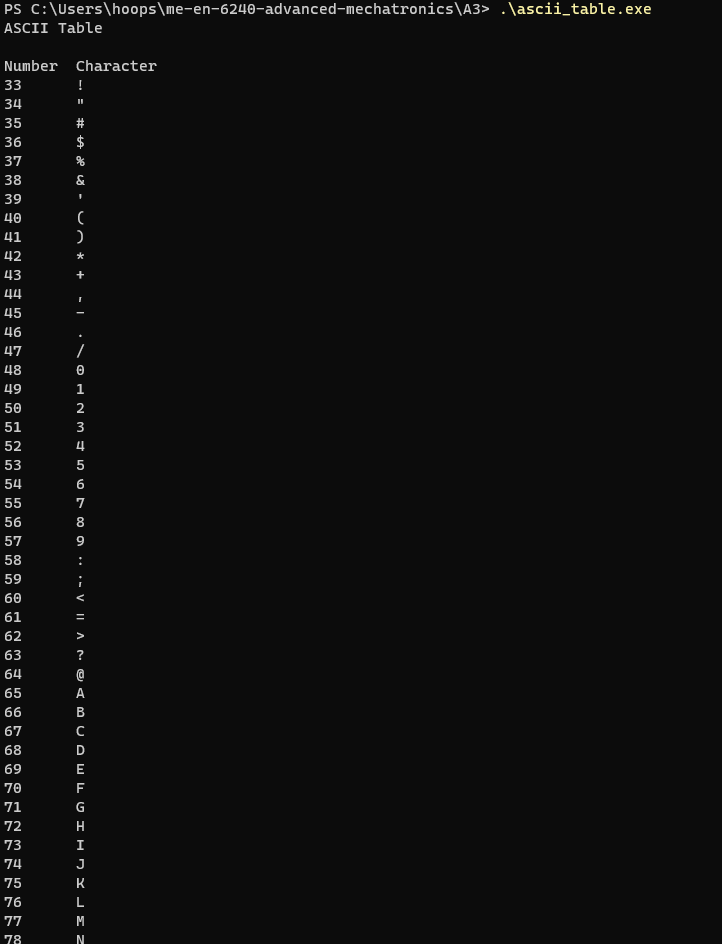
\includegraphics{ascii_table_img.png}
\end{center}

\subsection*{Exercise 35.}
See \verb|bubble.c|.

\vspace{.1in}
\begin{center}
    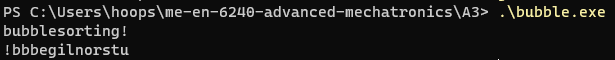
\includegraphics{bubble_sort_img.png}
\end{center}



\end{document}